\section{THE BACKGROUND OF VEDIC ASTROLOGY}
 

The following lesson introduces the student to the background issues of Vedic Astrology and the Vedic way of approaching astrology, applying it, and what the karmas involved may be, both for the client and the astrologer.

 

\subsection{SYSTEMS OF ASTROLOGY – EAST AND WEST}
 

Vedic Astrology is a “sidereal” astrology. This means that it uses the sidereal zodiac or the zodiac of the fixed stars. In this regard, it differs from most Western Astrology, which employs the “tropical zodiac” or the zodiac of the equinoxes. The two zodiacs are currently around 24 degrees apart according to the Ayanamsha used, with the Vedic sidereal zodiac falling behind the tropical zodiac.

 

To put it simply the tropical zodiac always begins the zodiac with the point of the vernal or spring equinox as representing the beginning of the sign Aries. The sidereal zodiac calculated the beginning of the sign Aries from a  certain point in the fixed stars. As the point of the equinox is moving backwards in the zodiac over time, the different between these two systems is now considerable and the calculations of planetary positions relative to them will vary by nearly one sign. While the sidereal zodiac of the fixed stars that Vedic astrology used can be viewed against the actual constellations in the sky, the tropical zodiac is a mathematical abstraction that cannot be seen in the sky as its boundaries are changing over time.

 

In general terms, we refer to Vedic astrology as sidereal and western astrology as tropical as these are the dominant systems. There is, however, a “Western Sidereal Astrology” introduced in the early twentieth century, which uses the sidereal zodiac but otherwise follows the aspects, house orientation and other methods of Western Tropical astrology. This is the basis of the “Fagan-Bradley” system. It arose through the influence of Vedic Sidereal astrolo­gy, but also argues that the original Western Astrology was a sidereal system. We may, therefore, call Vedic Astrology “Eastern Sidereal Astrology” but as Vedic Astrology is a simpler term.

 

There are also a few Vedic astrologers who use Vedic principles relative to the tropical zodiac, or who even claim that the original Vedic zodiac was tropical, but their numbers are very few, and they are not endorsed by the majority astrological community in India.  We find that view to be unfounded and misleading as Vedic texts for thousands of years have pointed out the shifting positions of the equinox and solstice points relative to the fixed stars.

 

In any case, different systems of astrology like different systems of healing are possible, and their principles can be different. Here we are aiming at classical Vedic astrology such as has dominated in India for many centuries and is sidereally based. We are not saying other systems may not have their value. However, there is only one zodiac and we find dividing it according to the fixed stars makes more sense as a way of understanding stellar influences, than dividing it by the equinoxes.

 



 

 

\subsection{THE ASTROLOGER AS LIFE-COUNSELOR}
 

The astrologer functions as a “life-counselor,” able to address all domains of life, including health, psychology, career, relation­ship, and spiritual issues. The field of astrology is the field of life itself. There is probably no other field that has such a broad scope of applications. The astrologer can specialize in one area but needs to know something of the whole of life. Astrol­ogy shows us the basic energetics of our lives in all their different dimensions. Some astrologers may take more limited roles or simply aim at providing information, not advice. But we feel that the life-counselor model is more useful and a better basis for practice, particularly in the West.

 

To be an astrologer, therefore, can be a more holistic career than to be a  psychologist or therapist of any kind. It requires a breadth of view and capacity to contemplate life as a whole. It may be the ultimate holistic occupation. To really do Vedic Astrology requires an integral approach and pyramidal vision, such as is revealed in the system of Vedic Science that covers all aspects of life. The astrologer should guide his or her client through the domains of life toward the full unfoldment of the soul, not through giving rigid directions or predictions but through pointing out the full scope of the clients potentials along with practical tools for developing their energies properly.

 

The astrologer should therefore study Yoga, Ayurveda and related Vedic subjects in order to be competent in this comprehensive approach. It is not necessary to master all of these subjects before attempting astrological readings, but one should gradually learn their fundamentals. Some astrologers possess much knowledge intuitively. Others bring it forward from different kinds of learning that they have already done.

 

Good astrological knowledge itself may not be enough to be a good astrologer. Just because we can see how the stars affect people or when events may occur in their lives, this may not be enough to help them understand these events or use them properly. There may be those who are good astrologers in some way or another. They may have good predictive powers but they may be unable to guide anyone in the higher goals of life. This requires not only astrological knowledge but spiritual development and integrity. A Vedic Astrologer should themselves follow a spiritual discipline, practicing yoga, meditation, mantra or rituals daily, and leading a life of honesty and integrity.  Their aim should not be to seek wealth, fame or power but to be of genuine service to their clients.

 

\subsection{THREE MODELS OF VEDIC ASTROLOGY}
 

Several different models of astrology exist. Two commonly related methods in Vedic Astrology today are the “predictive” and “judgmental” systems. Some people identify Vedic Astrology with these as a rigid and deterministic system. This is a misunderstanding. Vedic Astrology is also a very important counseling system, though it does have its predictive value.

 

\subsubsection{1. PREDICTIVE ASTROLOGY}
 

Predictive astrology aims at predicting specific events in life. These are mainly mundane events such as the timing of marriage, birth of children, the time of death, onset of various diseases, accidents, financial gains or losses, times of good or bad fortune, even the times of renunciation or liberation on a spiritual level.

 

The predictive astrologer aims at being able to predict events as specifically as possible. To this end, he may use not only the birthchart but also divisional and horary charts. These predictions may extend into the world at large, predicting wars, earthquakes, election outcomes, economic trends, stock market activity and even the weather, which are all part of mundane astrology.

 

Predictive astrology is linked to the timing of events. It is concerned with planetary periods, progressed charts, transits, horary charts and electional astrology, where timing is most important. It studies how outer events reflect astrological patterns and predicts the timing of their fructification.

 

From the standpoint of predictive astrology, the skill of the astrologer is judged by the accuracy of his or her predictions. The astrologer becomes a kind of weatherman for astral influences in life. There is not always something spiritual about such skill, but it can be allied with deeper insight. Such knowledge does not necessarily show us how to rightly deal with these events in our lives, although it can be combined with that as well.

 

From the standpoint of Vedic Astrology, predictive ability is important in an astrologer and it is a skill that all Vedic astrologers should strive to develop. If we cannot determine the astrological influences behind the events of a person’s life, we may not be able to determine how they affect them at a deeper level. Such outer events allow us to verify the chart and reflect the accuracy of our chart interpretations. This does not mean that we must always be able to tell our clients when specific things will occur to them on a daily basis but that at least we should be able to show them the major trends of their lives. Actually predicting specific events in the future is very difficult and has its dangers as we may be interfering with a person’s own power of judgment.

 

The predictive side of Vedic Astrology is probably the best of any astrological system and affords it much value. Many people approach it for this alone, particularly people from India who have a more uncertain material life. But it should be used to help clients put the events of their lives in proper perspective, integrating it into a spiritual approach that shows them how to use these events for spiritual development. It should not degenerate in giving the person the view that their life is mapped out or that they are victims of fate. In addition, until one has spent many hours examining a person’s chart and subchart it is not possible to understand the short term trends and indications in the chart. A mere general life-reading cannot do this.

 

 

\subsubsection{2. JUDGMENTAL ASTROLOGY}
 

This form of astrology aims at judging the different aspects of the life and character of a person: Their health, longevity, career, finances, marital happiness, level of intelligence, stage of spiritual evolution, and so on. It is similar to the predictive method, but looks to general capacities rather than to specific events. Most importantly, it has an ethical or spiritual side that some people are sensitive about. Many people do not like to think that they can be judged from a chart or that there is any limitation to their fate or destiny. However, Vedic Astrology, with its karmic orientation, acknowledges the history of the soul and the opportunities and limitations of each person and integrates this insight into its system.

 

Judgmental astrology places a value judgment on astrological positions. Some aspects are said to be good or bad, some planetary combinations are said to make a person good or evil, or intelligent or stupid. It often has an implied moralism that we should be very careful about, as karma is full of mystery and different indications.

 

Astrology should be capable of providing helpful judgments in life. But these should not be simplistic or subjective. They should be based upon spiritual goals and should not exalt worldly success or outward happiness as being of ultimate value. For example, a chart may indicate disease. This, however, is not necessarily something bad. It does not necessarily mean that person did something evil in their last life for which they have to pay. Disease can be an important means of awakening the soul. Therefore judgments in astrology should be applied with discretion. While astrologically we can see trends and tendencies, we should never deny the freedom of the soul to awaken and transcend its karma inwardly, even when it cannot change it outwardly.

 

Both the Predictive and the Judgmental models of astrology can have a fatalistic note about them that inhibits taking control of our own lives. Predictive astrology tells what is going to happen to us, as if we had no free will in life. Judgmental astrology tells what our nature is, as if nothing could be done about it. If we apply them in too matter of fact a way, we will encourage a fatalistic attitude in our clients. They will take their good fortune or misfortune too seriously, with finality, and lose the capacity for creative and spiritual growth in life. They may feel insulted or degraded by negative judgments and predictions, or flattered by the positive ones. Neither response leads to right action in life.

 

This fatalism occurred in medieval Western Astrology that also was judgmental in nature.  It was linked to a culture that believed in the predestination of the soul, and in an eternal heaven and hell. Such fatalism cannot exist in the Vedic system which is based on karma. Karma is not fate or predestination. It is a law of cause and effect in which our present state is the result of our past actions. We create our own destiny but we do so through time, in which who we are today has already been shaped by what we did yesterday.

 

Vedic Astrology does recognize the limitations of past karma, which can be very difficult to overcome, but it also teaches us that we can change our future. The future is the result of present actions, just as the present is the result of past actions. Vedic Astrology therefore encourages individual effort, not passivity, which is why remedial measures are so important. That past actions have influenced our present state does not mean that we should just accept our condition as limited. It means that we should act in a way today so as to ensure a better future and a more positive forward movement of our karma.

 

This course does not limit itself to Predictive or Judgmental methods, though they are used within it. The Predictive method, if applied superficially, becomes too mundane in nature. It can turn the astrologer into a mere fortune-teller. It gives people the impression that their destiny in life is fixed and that a good astrologer can remove any mystery about what will happen to them.

 

We should add that prediction is easier in a fixed and traditional culture like India. In the modern West, many of these predictive rules fail. For example, the potential for divorce is much higher in western culture today. For this reason, the traditional Hindu rules of marriage do not always work on charts of people in the West. Hence, these rules must be altered. They can show ease or difficulty in relationship, but how that translates into marriage or divorce is conditioned by the time and by the culture.

 

The Judgmental method can be too harsh. It can deprive people of the capacity for growth. It can reinforce any negativity in the chart. Even if the outer chart has many weaknesses, it should never be forgotten that our inner Self and true Being inherently transcends the influences of time and space. This method is particularly dangerous with passive, self-negative types of people who easily believe what is told to them, and are ready to accept something negative about themselves. It often becomes a self-fulfilling prophecy.

 

Personally, I think there is undesirable karma in following these methods too strongly or rigidly. To tell a gullible person that they have certain limitations in life or that they will suffer some difficulty at a certain time may make it occur. The astrologer should act in such a way as not to deprive the client of his or her own power of judgment. The astrologer can give clients information or tools to work with but they must not take power over their clients. The astrologer is not God and the birthchart is seldom so fixed that all astrologers will interpret it in the same way. Therefore, the astrologer should not be too proud or convinced of his or her opinions. He should remain open to the fluidity of life. While we may have to warn our clients of the effects of wrong actions, this should stimulate them to a better way of living, not make them feel that they cannot change their condition.

 

There is yet another approach to Vedic Astrology that we should note. This is more the flattery method in which the astrologer tells the client everything good about them and their chart. It may be done in an effort to show people the positive side of their nature or it may just be done to gain more clients. If we do not point out the difficulties inherent in a chart, we are also doing our client a disservice. We should point these out in a way that enables the client to use them as a basis for greater growth and understanding. We should neither ignore them nor present them in a rigid manner. We should point out both the positive and the negative objectively and try to give the client the tools to use the higher potentials in their chart – and there is seldom a chart without them.

 

\subsubsection{3. SPIRITUAL ASTROLOGY AND ASTROLOGICAL COUNSELING}
 

The system taught in this course is more a form of spiritual astrology and astrological counseling. It uses astrology as a tool for self-knowledge and an aid in Self-realization. It uses the cosmic forces transmitted to us through the planets to connect us with our own deeper cosmic nature. In this regard, I always teach my clients the basic meaning of the planets in their charts and the characteristics of their planetary type. This allows them to enter into the process of astrological knowledge which is necessary for astrology to become a useful tool for self-growth.

 

It employs predictive and judgmental methods but in a broader spiritual context. I try to acquaint my clients with both the good and bad potentials of their chart and offer them the tools to augment the good and ward off the bad. I do not leave my clients victims of fate. I teach them that their soul transcends time and that it can use the energetics of the chart in several ways. I do not recognize an absolute fate in life but only probabilities that can be high, medium or low.  For example, I may tell a client their chart is not good for relationship or that it may be prone toward divorce, but I would be hesitant to tell them that marriage is impossible (though there are cases of this). I would hesitate to give a person the date of their divorce when a difficult period for marriage is indicated. However, I would inform them if a relationship were unlikely to endure through a given planetary period.

 

This approach does not aim at prediction alone. I am more concerned with helping the client to manage their planetary energies rather than merely telling them what is likely to befall them for good or ill. I relate to them favorable or unfavorable periods for different ventures or affairs and help them guide the course of their lives through these. I encourage them to action on all levels through the remedial measures of Vedic Astrology and its related systems of Yoga and Ayurveda. I believe that the proof of a good astrologer is how he or she makes their clients aware of their astral influences and how to better manage them, not how good he or she is at predicting particular events only. Such an approach is not aimed at making the individual more tied to his external nature but opens up the potentials of the spiritual life which the individual may not yet be using or even be aware of.

 

\subsection{THE ASTROLOGY OF HEALING/ YOGIC ASTROLOGY AND AYURVEDIC ASTROLOGY}

 

Astrology requires a healing method to be really useful. We must not only be able to recognize planetary influences in our lives; we need to know how to harmonize them. We must help our clients learn how to balance the planetary influences in their lives.

 

An astrology of healing has two levels: First, Vedic astrology has measures to treat our outer nature and, second, those to treat our inner nature. The outer nature, our body, senses and conditioned mind, can be treated by medical and psychological methods that are not specifically astrological in nature. Our inner nature, our soul, requires occult and yogic methods and ultimately rests upon our own effort to grow spiritually in life. This has more scope for astrological healing measures.

 

Vedic Astrology is not just a predictive or interpretative system.  It is also a remedial system with techniques and methods for balancing planetary influences. These are as essential as the interpretative side. What use is it to tell people what is going to happen to them if we cannot give them a means of dealing with it? For this reason, the second part of this course includes such remedial measures as gems, mantras, yantras, herbs, and color therapy, and the role of Ayurveda as well as Yoga.

 


\subsection{THE FOUR AIMS OF LIFE}
 

On this foundation of examining the different models and goals for Vedic astrology we will now introduce the Vedic view of life. Vedic Science traditionally recognizes four legitimate aims or goals of human life: Dharma, Artha, Kama and Moksha.

 

DHARMA means “principle or law” and refers to the fulfill­ment of our right purpose in life.  It includes the honor or recognition we attain through our actions on a personal and professional level, specifically through the medium of career. It relates to broader principles of truth and right action. Ultimately it refers to our soul’s purpose in this incarnation.
ARTHA means “achievement of goals” and relates specifically to the acquisition of material resources required to fulfill ones dharma in life.  It relates to income and wealth.
KAMA means literally “desire” and refers to our need for emotional and sensory happiness. As such, we could call it “enjoyment.” But lasting happiness is only possible when we fulfill our dharma.
MOKSHA means “freedom” or liberation and relates to our need for spiritual growth, including transcendence of the above three lower values.
 

Vedic Astrology recognizes the validity of all four aims and is oriented to facilitate the human being in the attainment of each of them. Yet in Vedic Science the first three, career, wealth and enjoyment are subordinate to the last, spiritual liberation. Liberation is the primary and essential goal for all human beings. Without it, the other goals have no real meaning. The others are merely a support for it and have no validity in themselves. An astrologer using the Vedic system should, therefore, give a comprehensive view of all the domains of life. Yet he should focus on liberation and the spiritual life. This does not mean to take the role of a guru but to show the higher usages that can be made of the planetary energies and circumstances in ones life.

 

From the Vedic perspective, a chart that is good for liberation but not for the other domains of life is a much better chart to have than one that is good for the lesser goals but not for the spiritual life.

 

As a foundation for the four aims of life, astrology addresses the need for health, arogya, or freedom from disease. This is the basis for the four aims of life, for without health, what else can be accompli­shed? Yet health is not just physical, it is also mental. So astrology must consider physical and mental health or physical health and psychological well‑being as the means of approaching all the goals of life. Hence, medical and psychological astrology, after spiritual astrology, are its most important branches.

 

I have addressed some of the astrological indications of these factors. These will be more understandable later on in the course.

 

 

\subsubsection{DHARMA}

 

Dharma refers in a broader sense to the spiritual principles and natural laws that govern the universe. In the individual context it refers to our basic nature, inclinations and capacities in life. Dharma as career, refers to right vocation and the happiness inherent in fulfilling ones capacities for right action in life. Ones true Dharma is that of ones soul, our hearts vocation, not what society imposes upon us. Yet most of what we call Dharma is revealed by our occupation in life, how we earn our livelihood.

 

Under this concept are also included honor, position, status, fame, prestige and power. These show our social dharma and its effects, including how our character affects the world. Our individual dharma should reflect in some way the universal dharma. If our dharma is adharmic; that is, if our career is harmful to others, then it will end up harming ourselves as well.

 

Dharma is related to Artha, the objects and goals that we seek to attain things in life. Usually it is through our career that we seek wealth.

 

 

\subsubsubsection{Indications in the Chart}

 

These indications will make more sense later in the course after students are more familiar with the planets. Please remember it for future reference.

 

Jupiter, Mercury and the Sun are the main planets that rule Dharma. Mercury shows how we function and communicate in society. Jupiter shows the role or law we like to follow in life, our guiding principles and the goals we seek. The Sun shows our ability to project our character and personality, the influence of our nature on the world.

 

Dharma houses are the first, which shows our personal dharma and responsibility to self, the fifth which shows our creative dharma and responsibility to children, and the ninth that shows our spiritual and social dharma.

 

For house influences, we should note that of the first, ninth and tenth houses and their lords. The first tells us who we are generally; it is the measure of our identity and action in the world. The ninth shows the goals or profession we aspire to. The tenth measures our capacity to impact the world karmically. It shows how our personality appears in the world. It shows how our dharma achieves artha, or value, both for ourselves and for society.

 

 

\subsubsection{ARTHA}

 

Artha, wealth, refers to all necessary means of material livelihood and security, not simply the pursuit of material gain. The astrologer should be able to counsel his clients on how to best use their material potential in life. This is in directing it towards spiritual or dharmic ends, not simply pursuing money for the power or status that it may afford.

 

 

\subsubsubsection{Indications in the Chart}

 

The planets that rule Artha are Jupiter and Mercury. Jupiter governs our capacity for gains and abundance generally. Mercury rules our ability for commerce and exchange. Venus also gives wealth and comfort, art or luxury. Saturn tends to create poverty (though it can give us property and other hard or fixed assets).

 

Houses of artha are the second, sixth and tenth. The second shows how we gain our personal livelihood. The sixth shows work capacity and money from sources such as insurance or legal settlements. The tenth shows career gains, staus and achievement.

 

In particular, we should take into account the influences on the second and eleventh houses and their lords. The second governs our ability to earn through our own labor, the eleventh to gain income from various sources. After these we should consider the fourth, fifth and ninth houses and their lords, which all give wealth. The fourth gives property and vehicles. The fifth gives gain through counseling, advice and speculation, like the stock market. The ninth gives grace and fortune, like the winning of lotteries.

 

The twelfth, sixth and eighth houses and their rulers tend to limit wealth. The twelfth shows loss and expenses. This in itself may not create poverty if the houses of income are strong. The sixth gives loss through disease, enmity, legal problems, overwork or lack of recognition. The eighth shows difficulties, obstacles, oppression, lack of recognition or bad reputation.

 

 

\subsubsection{KAMA}

 

Kama, enjoyment, refers to all legitimate sensory enjoyments, not just pleasure in the gross sense but the enjoyments natural to the right use of the senses. To enjoy life, to appreciate the beauty of nature, true art and loving communication between human beings, is part of the fulfillment of our soul and need not be denied for spiritual growth. In fact, all life is a seeking of happiness. It springs from joy itself. If we were not in some way happy or able to find happiness, why would we wish continue living?

 

Our enjoy­ment or pleasure in life is largely through relationship, which includes sexuality. Hence, relationship is the main factor of Kama and its issues of love, marriage, partnership and children. The higher level of Kama or enjoyment relates to our artistic sense. The highest level relates to our capacity for devotion, our openness to Divine love, beauty and delight.

 

 

\subsubsubsection{Indications in the Chart}

 

The planet that rules Kama is Venus, the planet of desire. According to its position in the chart, our capacity for enjoyment or Kama can be read. Mars is also important as it shows our goal-seeking in life. Aligned to Venus, it often takes us along the realm of desire. Jupiter gives us capacity for enjoyment or happiness of a more general nature, while Saturn tends to deny or limit it. Saturn aligned with Mars may cause us to seek perverted or unwholesome means of enjoyment.

 

Kama houses are three, seven and eleven. The third is the house of talents, hobbies, curiosities, interests and sports – personal kama. The seventh house is the house of love, marriage and fulfillment in human relationship – relationship kama. The eleventh is the house of friendship, expression, social and career gains – social kama. The fifth is also important as the house of romance, joy and creativity, the happiness that comes from dharma. The twelfth is the house of secret pleasures and hidden desires and has some relevance as well and also indicates the happiness that comes from moksha.

 

 

\subsubsection{MOKSHA}

 

Moksha, liberation, refers to our work of Self‑realization in life, our efforts at Self‑knowledge. It includes whatever liberates our inner spirit and creative force in life. In its proper domain, it transcends organized religion and codified beliefs and is ultimately an individual affair.

 

The pursuit of various forms of knowledge, including philosophy, science and the occult, as well as creative expression, like art, are themselves lesser aspects of the goal of liberation. For this reason, the aim of liberation can also be defined as knowledge. All of us are seeking knowledge or freedom in one way or another. It is knowledge that gives us freedom, which extends our horizons and gives us access to the greater world beyond the limits of our body and senses. Yet knowledge may be lower, as of the outer world, or higher, as of the true Self. This latter is the real goal through which real liberation is possible. The lesser knowledge gives us greater space to operate in the world but it does not free us from the limitations of worldly existence.

 

 

\subsubsubsection{Indications in the Chart}

 

Jupiter and Ketu rule Moksha. Jupiter shows our general seeking of expansion and truth, our aspiration and need to grow and transcend. Ketu shows our ability to negate and transcend things. It affords deep insight, discrimination and perception. Saturn is also important as it gives detachment, renunciation and the capacity to be alone. Mercury is important, as the indicator of the intellect; it shows the level of knowledge that we seek.

 

Houses of Moksha are fourth, eighth and twelfth. The fourth shows our emotional happiness. The eighth shows occult and mental insight. The twelfth shows spiritual liberation.

 

The house influences of the ninth and twelfth together are important, as well as their lords, with Jupiter the significator of the ninth and Ketu of the twelfth. The ninth gives us our sense of values, goals, principles and aspirations. It shows the dharma behind our pursuit of moksha. The twelfth allows us to negate our experiences and go beyond what we already are (our conditioned being). It also shows the past and the latent impressions in the subconscious that motivates us. The fifth house has some importance as the measure of the good karma we bring into the present life, the indication of past spiritual practices. It also shows our devotion in life, what form or energy of the Divine that we seek.

 

The fourth and eighth houses also relate to liberation. The fourth shows our capacity for peace of mind, the foundation of all spiritual pursuits. It shows self-contentment, psychological stability and mental receptivity. The eighth shows our ability to go beyond death and time, the gateway to the eternal. It gives the ability to transcend suffering and often affords deep perception.

 

The planets of ignorance and attachment often limit our pursuit of Moksha. These are particularly Venus and Mars, the planets of passion and sexuality. Saturn can provide the detachment that aids us in liberation or it can create darkness of mind that prevents it. Jupiter can get us attached to outer affluence or religious ceremonialism. Hence, liberation is the most complex thing to measure in a chart. All planets have a higher or spiritual and lower or materialistic functioning.

 

Jupiter, as the great benefic, is the planetary indicator of our positive goals in life. So it is the most important planet in showing how we can achieve any of the four aims of life. How our Jupiter is oriented will show the areas in which we will seek our highest good in life.

 

Saturn, as the indicator of karma or destiny, shows the limitations we encounter but is also useful in giving us the lesson of suffer­ing that takes us from the lower to the higher goals.

 

When both Jupiter and Saturn balance each other and further spiritual knowledge, we are able to attain our maximum destiny in life and become a person of true greatness.

 

The lunar nodes have a similar importance. Rahu, the north node, shows where we are apt to overly project ourselves into the outer world. Ketu, the south node, indicates where we are prone to overly contract ourselves into the inner world. When the lords of both nodes are in harmony our lives function well. When they are in harmony on a spiritual level, great transformation is possible.

 

\subsubsection{Relationship between the Four Aims of Life}

 

These four aims are like a pyramid with liberation at the top. Each is meant to aid in the others. We need to be happy generally in order to function at all. We need the resources to enable us to have leisure and peace of mind. We need the acknowledgment or recognition of others. In this regard, a failure or inability to achieve the lower goals can inhibit the higher. If we are impoverished, degraded, ill or stupid, it is difficult to get beyond the outer aspects of life.

 

Yet most of us are caught in the lower goals and do not appreciate the higher in our true nature. Often our pursuit of the higher remains a pursuit of the lower in disguise. In the name of God, we still seek pleasure, power or fame. Astrology is also usually denigrated in such a way when its lower rather than higher insights are implemented.

 

It is important not to deny the pursuit of any of these aims for anyone but to show how they relate properly to and direct us toward the true goal of spiritual liberation. We should never encourage a client to pursue these outer goals as the highest pursuit in life. There may be times in life when it is necessary to focus on them or take advantage of the favorableness of the time to achieve them, but this can be done with a long-term spiritual orientation. For this reason, we should not give the lower goals too much weight in reading a chart. A purely business astrology, for example, would not be in harmony with the Vedic approach unless the business was oriented towards spiritual goals.

 

When we define success or failure, difficulty or ease for people based upon their charts, we must indicate in which domain and on what level. We may judge a chart as good for wealth or career, but this does not mean it is good for health or spirituality. In this way, many charts that are difficult for ordinary goals have higher blessings.

 

\subsubsection{THE KARMA OF AN ASTROLOGER}

 

The modern world does not believe in karma, but in money and the fame that the world gives us. There is the tendency to think that if our work gives us wealth and recognition then it is good. This, however, may not be the case. As wealth and recognition are outer values, they can come to us according to an outer or unspiritual orientation in life. Astrology can give wealth and fame but also deeper knowledge. The two are neither inclusive or exclusive of each other but the latter is the real grace of astrology through which alone true happiness will come to us.

 

To do Vedic Astrology properly, we must teach our clients the laws of karma and live according to them ourselves as well. Vedic astrology is the ultimate system of karmic management, both for ourselves and others. It is not our name and wealth that we take with us when we die but our karma. It is our main purpose in life to reduce our karmic burden and aid others in doing so. This is also the true role of the astrologer. A worldly astrology that flatters people, that encourages them to seek happiness in the outer world, that glorifies wealth, fame and talent, breeds more karma for the astrologer and their clients.

 

As astrology is an intimate form of counseling and deals with the deepest issues of life, it carries great responsibility. It has a power that can work against us if we apply it in the wrong manner. If we give our clients wrong advice or project them in a direction that may not be helpful to their soul, then it will be our karma to similarly be misdirected by others or to misdirect ourselves. Even if a chart is very good for outer things like wealth, we should not simply glorify such good fortune for our client but show its limitations. Similarly, if a chart is not good for the outer goals of life, we should point the positive value of such a chart for bringing us into the spiritual life.

 


\subsection{\textbf{Talk by Dr. David Frawley on Vedic Astrology and Vedic Counseling
Shows how we view and apply Vedic astrology in our integral approach to Vedic knowledge}}

\begin{figure}[H]
 \centering
\includegraphics[width=0.8\textwidth]{pics/overview1.png}
 \end{figure}

\begin{figure}[H]
 \centering
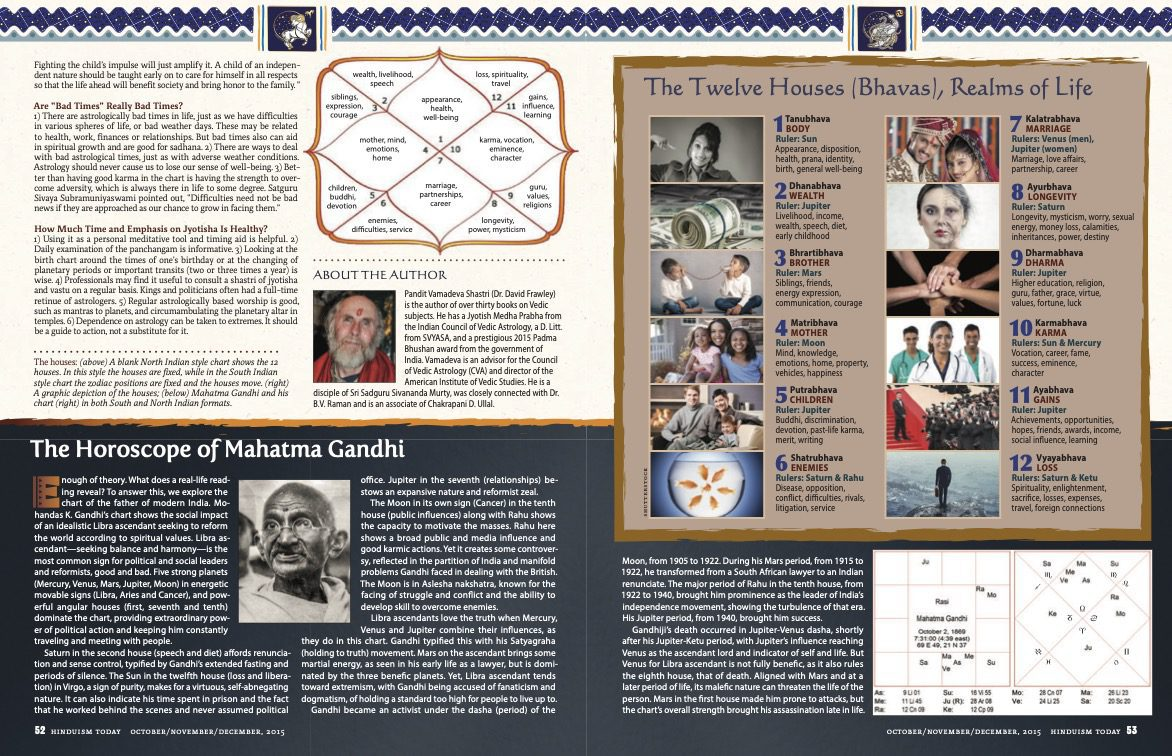
\includegraphics[width=0.8\textwidth]{pics/overview2.png}
 \end{figure}

